\chapter{Finden von wichtigen / interessanten Stellen im Code}

Minimalismus ist kein beliebtes Feature moderner Software.

\myindex{\Cpp!STL}

Aber nicht weil die Programmierer so viel Code schreiben, sondern weil die Libaries
allgemein statisch zu ausf\"uhrbaren Dateien gelinkt werden. Wenn alle externen
Libraries in externe DLL Dateien verschoben werden w\"urden, w\"are die Welt ein
anderer Ort. (Ein weiterer Grund f\"ur C++ sind die \ac{STL} und andere Template-Libraries.)

\newcommand{\FOOTNOTEBOOST}{\footnote{\url{http://www.boost.org/}}}
\newcommand{\FOOTNOTELIBPNG}{\footnote{\url{http://www.libpng.org/pub/png/libpng.html}}}

Deshalb ist es sehr wichtig den Ursprung einer Funktion zu bestimmen, wenn die
Funktion aus einer Standard-Library oder aus einer sehr bekannten Library stammt
(wie z.B Boost\FOOTNOTEBOOST, libpng\FOOTNOTELIBPNG), oder ob die Funktion sich
auf das bezieht was wir im Code versuchen zu finden.

Es ist ein wenig absurd s\"amtlichen Code in \CCpp neu zu schreiben, um das zu
finden was wir suchen.

Eine der Hauptaufgaben eines Reverse Enigneers ist es schnell Code zu finden den
er/sie sucht.

\myindex{\GrepUsage}

Der \IDA-Disassembler erlaubt es durch Textstrings, Byte-Sequenzen und Konstanten
zu suchen.  Es ist sogar m\"oglich den Code in .lst oder .asm Text Dateien zu
exportieren und diese mit \TT{grep}, \TT{awk}, etc. zu untersuchen.

Wenn man versucht zu verstehen wie ein bestimmter Code funktioniert, kann auch
eine einfache Open-Source-Library wie libpng als Beispiel dienen.
Wenn man also eine Konstante oder Textstrings findet die vertraut erscheinen, ist
es immer einen Versuch wert diese zu \emph{google}n .
Und wenn man ein Opensource Projekt findet in dem diese Funktion benutzt wird, 
reicht es meist aus diese Funktionen miteinander zu vergleichen.
Es k\"onnte helfen Teile des Problems zu l\"osen.

% When you try to understand what some code is doing, this easily could be some open-source library like libpng.
% So when you see some constants or text strings which look familiar, it is always worth to \emph{google} them.
% And if you find the opensource project where they are used, 
% then it's enough just to compare the functions.
% It may solve some part of the problem.

Zum Beispiel, wenn ein Programm XML Dateien benutzt, w\"are der erste Schritt zu ermitteln welche
XML-Library benutzt wird f\"ur die Verarbeitung, da die Standard (oder am weitesten verbreitete) libraries
normal benutzt werden anstatt selbst geschriebene librarys.

\myindex{SAP}
\myindex{Windows!PDB}

Zum Beispiel, der Autor dieser Zeilen wollte verstehen wie die Kompression/Dekompression von Netzwerkpaketen in SAP 6.0 funktioniert.
SAP ist ein gewaltiges St\"uck Software, aber detaillierte -\gls{PDB} Dateien mit Debug Informationen sind vorhanden, was sehr praktisch 
ist. Der Autor hat schließlich eine Ahnung gehabt, das eine Funktion genannt \emph{CsDecomprLZC} die Dekompression der Netzwerkpakete \"ubernahm.
Er hat nach dem Namen der Funktion auf google gesucht und ist schnell zum schluss gekommen das diese Funktion in 
MaxDB benutzt wurde (Das ist ein Open-Source SAP Projekt) \footnote{Mehr dar\"uber in der relevanten Sektion~(\myref{sec:SAPGbUI})}. 

\url{http://www.google.com/search?q=CsDecomprLZC}

Erstaunlich, das MaxDB und die SAP 6.0 Software den selben Code geteilt haben f\"ur die Kompression/Dekompression der Netzwerkpakete.

\mysection{Ausf\"uhrbare Dateien Identifizieren}

\subsection{Microsoft Visual C++}
\label{MSVC_versions}

MSVC Versionen und DLLs die Importiert werden k\"onnen:

%\small
\begin{center}
\begin{tabular}{ | l | l | l | l | l | }
\hline
\HeaderColor Marketing ver. & 
\HeaderColor Internal ver. & 
\HeaderColor CL.EXE ver. &
\HeaderColor DLLs imported &
\HeaderColor Release date \\
\hline
% 4.0, April 1995
% 97 & 5.0 & February 1997
6		&  6.0	& 12.00	& msvcrt.dll	& June 1998		\\
		&	&	& msvcp60.dll	&			\\
\hline
.NET (2002)	&  7.0	& 13.00	& msvcr70.dll	& February 13, 2002	\\
		&	&	& msvcp70.dll	&			\\
\hline
.NET 2003	&  7.1	& 13.10 & msvcr71.dll	& April 24, 2003	\\
		&	&	& msvcp71.dll	&			\\
\hline
2005		&  8.0	& 14.00 & msvcr80.dll	& November 7, 2005	\\
		&	&	& msvcp80.dll	&			\\
\hline
2008		&  9.0	& 15.00 & msvcr90.dll	& November 19, 2007	\\
		&	&	& msvcp90.dll	&			\\
\hline
2010		& 10.0	& 16.00 & msvcr100.dll	& April 12, 2010 	\\
		&	&	& msvcp100.dll	&			\\
\hline
2012		& 11.0	& 17.00 & msvcr110.dll	& September 12, 2012 	\\
		&	&	& msvcp110.dll	&			\\
\hline
2013		& 12.0	& 18.00 & msvcr120.dll	& October 17, 2013 	\\
		&	&	& msvcp120.dll	&			\\
\hline
\end{tabular}
\end{center}
%\normalsize

msvcp*.dll hat \Cpp{}-bezogene Funktionen, bedeutet wenn die library importiert wird,
ist das Programm das sie importiert wahrscheinlich ein \Cpp program.

\subsubsection{Name mangling} 

Die Namen fangen normal an mit dem \TT{?} Symbol.

Hier: \myref{namemangling} kann man mehr lesen \"uber MSVC's \gls{name mangling} . 

\subsection{GCC}
\myindex{GCC}

Neben *NIX Umgebungen, ist GCC auch in win32 Umgebungen pr\"asent, in der Form von Cygwin and MinGW. 

\subsubsection{Name mangling} 

Namen fangen hier normal mit dem \TT{\_Z} Symbolen an.

Man kann mehr lesen \"uber GCC's \gls{name mangling} hier: \myref{namemangling}.

\subsubsection{Cygwin}
\myindex{Cygwin}

cygwin1.dll wird oft importiert.

\subsubsection{MinGW}
\myindex{MinGW}

msvcrt.dll wird vielleicht importiert.

\subsection{Intel Fortran}
\myindex{Fortran}


libifcoremd.dll, libifportmd.dll and libiomp5md.dll (OpenMP Support) werden vielleicht importiert.

libifcoremd.dll hat eine menge an Funktionen die das \TT{for\_} Pr\"afix haben, was \emph{Fortran} bedeutet.

\subsection{Watcom, OpenWatcom}
\myindex{Watcom}
\myindex{OpenWatcom}

\subsubsection{Name mangling}

Namen fangen normal mit dem \TT{W} Symbol an. 

Zum Beispiel wird so eine Methode benannt \q{method} der Klasse \q{class} die keine Argumente hat und \Tvoid zur\"uck gibt: % <-- Finde was besseres!
% For example, that is how the method named \q{method} of the class \q{class} that does not have any arguments and returns
% \Tvoid is encoded:

\begin{lstlisting}
W?method$_class$n__v
\end{lstlisting}

\subsection{Borland}
\myindex{Borland Delphi}
\myindex{Borland C++Builder}

Hier ist ein Beispiel f\"ur Borland Delphi's und C++Builder's \gls{name mangling}:

\lstinputlisting{digging_into_code/identification/borland_mangling.txt}

Die Namen fangen immer mit dem \TT{@} Symbol an, dann haben wir den Namen
der Klassen Namen, Methoden Namen, und codiert die Typen der Argumente der Methode.

Diese Namen k\"onnen in den .exe Imports, .dll Exports, Debug Daten und etc existieren.

Borland Visual Component Libraries (VCL) 
werden in .bpl Dateien gehalten anstatt .dll's, zum Beispiel vcl50.dll, rtl60.dll.

Eine weitere DLL die vielleicht importiert wird: BORLNDMM.DLL

\subsubsection{Delphi}

Fast alle Delphi executables haben den \q{Boolean} Text String am Anfang des Code Segments, zusammen mit den Namen anderer Typen liegen.
% Almost all Delphi executables has the \q{Boolean} text string at the beginning of the code segment, along with other type names.

Dies ist ein sehr typischer Anfang f\"ur das \TT{CODE} Segment bei einem 
Delphi Programm, dieser Block kam direkt nach dem win32 PE Datei header:

\lstinputlisting{digging_into_code/identification/delphi.txt}

Die ersten 4 Btyes des Daten Segments (\TT{DATA}) k\"onnen \TT{00 00 00 00}, \TT{32 13 8B C0} oder \TT{FF FF FF FF} sein.

Diese Informationen k\"onnen n\"utzlich sein wenn man mit gepackten oder verschl\"usselten Delphi executables arbeiten muss. 

\subsection{Other known DLLs}

\myindex{OpenMP}
\begin{itemize}
\item vcomp*.dll---Microsoft's Implementierung von OpenMP. 
\end{itemize}

 

\mysection{Kommunikation mit der außen Welt (Funktion Level)} 
Oft ist es empfehlenswert die Funktionsargumente und die R\"uckgabewerte im
Debugger oder \ac{DBI} zu \"uberwachen. Zum Beispiel hat der Autor einmal
versucht die Bedeutung einer obskuren Funktion zu verstehen, die einen inkorrekten
Bubblesort-Algorithmus implementiert hatte\footnote{\url{https://yurichev.com/blog/weird_sort_KLEE/}}
(Sie hat funktioniert, jedoch viel langsamer als normal). Die Eingaben und Ausgaben zur Laufzeit 
der Funktion zu \"uberwachen hilft sofort zu verstehen was die Funktion tut.

% TBT

% sections:
\mysection{Kommunikation mit der Außen Welt (Win32)}

Manchmal reicht es die Ein- und Ausgaben einer Funktion zu beobachten um zu verstehen was sie tut.
Auf diese Weise kann man Zeit Sparren.

Datei und Regestry Zugriff:
F\"ur einfache Analysen kann das Tool Prozess Monitor\footnote{\url{http://technet.microsoft.com/en-us/sysinternals/bb896645.aspx}}
von SysInternals hilfreich sein.

Bei einfachen Netzwerk Zugriffen ist Wireshark\footnote{\url{http://www.wireshark.org/}} zum analysieren ganz n\"utzlich.

Trotzdem muss man einen Blick in die Netzwerkpakte werfen.
\\
Das erste wonach man schauen kann ist welche Funktionen die \ac{OS} \ac{API}s benutzen und was f\"ur Standard libraries
benutzt werden. 

Wenn das Programm unterteilt ist in eine Main executable und mehrere DLL Dateien, k\"onnen manchmal die Namen der Funktionen innerhalb
der DLLs Helfen. 

Wenn wir daran interessiert sind was genau zum Aufruf von \TT{MessageBox()} mit einem spezifischen Text f\"uhrt,
k\"onnen wir versuchen diesen Text innerhalb des Data Segments zu finden, die Referenzen auf den Text und die 
Punkte von denen aus die Kontrolle an den \TT{MessageBox()} Aufruf an dem wir interessiert sind. %<--- Das muss verständlicher geschrieben werden.

\myindex{\CStandardLibrary!rand()}
Wenn wir \"uber Video Spiele sprechen sind wir daran interessiert welche \rand aufrufe mehr oder weniger zuf\"allig darin vorkommen,
vielleicht versuchen wir die \rand Funktion oder Ersatz Funktionen zu finden ( wie z.B der Mersenne Twister Algorithmus) 
und wir versuchen die Orte zu finden von welchen aus diese Funktionen aufgerufen werden, und noch wichtiger was f\"ur
Ergebnisse verwertet werden. 
% BUG in varioref: http://tex.stackexchange.com/questions/104261/varioref-vref-or-vpageref-at-page-boundary-may-loop
Ein Beispiel: \myref{chap:color_lines}.

Aber wenn es sich nicht um ein Spiel handelt und \rand wird trotzdem benutzt, ist es interessant zu wissen warum.
Es gibt F\"alle bei denen unerwartet \rand in Daten Kompressions Algorithmen benutzt wird (f\"ur die Imitation von Verschl\"usslung):
\href{http://blog.yurichev.com/node/44}{blog.yurichev.com}.

\subsection{Oft benutzte Funktionen in der Windows API}

Diese Funktionen sind vielleicht unter den importierten.
Es ist Sinnvoll an dieser Stelle zu erw\"ahnen das nicht unbedingt jede Funktion benutzt wird aus 
dem Code den der Programmierer geschrieben hat.

Manche Funktionen haben eventuell das \GTT{-A} Suffix f\"ur die ASCII Version und das \GTT{-W} f\"ur die Unicode Version.


\begin{itemize}

\item
Registry zugriff (advapi32.dll): 
RegEnumKeyEx, RegEnumValue, RegGetValue, RegOpenKeyEx, RegQueryValueEx.

\item
Zugriff auf text .ini-files (kernel32.dll): 
GetPrivateProfileString.

\item
Dialog boxes (user32.dll): 
MessageBox, MessageBoxEx, CreateDialog, SetDlgItemText, GetDlgItemText.

\item
Resourcen zugriff (\myref{PEresources}): (user32.dll): LoadMenu.

\item
TCP/IP networking (ws2\_32.dll):
WSARecv, WSASend.

\item
Datei Zugriff (kernel32.dll):
CreateFile, ReadFile, ReadFileEx, WriteFile, WriteFileEx.

\item
High-level Zugriff auf das Internet (wininet.dll): WinHttpOpen.

\item
Die digitale Signatur einer ausf\"uhrbaren Datei pr\"ufen (wintrust.dll):

WinVerifyTrust.

\item
Die Standard MSVC library ( wenn sie dynamisch gelinked wurde) 

assert, itoa, ltoa, open, printf, read, strcmp, atol, atoi, fopen, fread, fwrite, memcmp, rand,
strlen, strstr, strchr.

\end{itemize}

\subsection{Verl\"angerung der Testphase}

Registry Zugriffs Funktionen sind h\"aufig ziele f\"ur Leute die versuchen die Testphase einer Software zu cracken, die 
eventuell die Installations Zeit und Datum in der Regestry zu speichert. 

Ein weiteres beliebtes Ziel sind die GetLocalTime() und GetSystemTime() Funktionen:
eine Test Software, muss bei jedem Start die aktuelle Zeit und Datum \"uberpr\"ufen.

\subsection{Entfernen nerviger Dialog Boxen}

Ein verbreiteter Weg raus zu finden was eine dieser nervigen Dialog boxen macht, ist den 
Aufruf von MessageBox(), CreateDialog() und CreateWindow() Funktionen abzufangen.


\subsection{tracer: Alle Funktionen innerhalb eines bestimmten Modules abfangen}

\myindex{tracer}

\myindex{x86!\Instructions!INT3}
Es gibt INT3 breakpoints in \tracer, die nur einmal ausgel\"ost werden. Jedoch k\"onnen diese breakpoints f\"ur alle 
Funktionen in einer bestimmten DLL gesetzt werden.

\begin{lstlisting}
--one-time-INT3-bp:somedll.dll!.*
\end{lstlisting}

Oder, lasst uns einfach mal INT3 breakpoints f\"ur alle Funktionen setzen, die das \TT{xml} Pr\"afix in ihrem Namen haben:

\begin{lstlisting}
--one-time-INT3-bp:somedll.dll!xml.*
\end{lstlisting}

Die andere Seite der Medaille ist, solche breakpoints werden nur einmal ausgel\"ost.
Tracer zeigt den Aufruf der Funktion, wenn er passiert, aber auch nur einmal. 
Ein weiterer Nachteil ist---es ist unm\"oglich die Argumente der Funktion zu betrachten.

Dennoch, dieses Feature ist sehr n\"utzlich wenn man weiß das das Programm eine DLL benutzt,
aber man nicht weiß welche Funktionen aufgerufen werden. Und es gibt eine ganze Menge an 
Funktionen.


\par
\myindex{Cygwin}
Zum Beispiel, schauen wir uns einmal an was das uptime Kommando aus cygwin benutzt:

\begin{lstlisting}
tracer -l:uptime.exe --one-time-INT3-bp:cygwin1.dll!.*
\end{lstlisting}

Dadurch sehen wir alle cygwin1.dll library Funktionen die zumindest einmal aufgerufen wurden, und von welcher
Stelle: 
\lstinputlisting{digging_into_code/uptime_cygwin.txt}


\mysection{Strings}
\label{sec:digging_strings}

\mysection{x86}

\subsection{Terminologie}

Geläufig für 16-Bit (8086/80286), 32-Bit (80386, etc.), 64-Bit.

\myindex{IEEE 754}
\myindex{MS-DOS}
\begin{description}
	\item[Byte] 8-Bit.
		Die DB Assembler-Direktive wird zum Definieren von Variablen und Arrays genutzt.
		Bytes werden in dem 8-Bit-Teil der folgenden Register übergeben:
		\TT{AL/BL/CL/DL/AH/BH/CH/DH/SIL/DIL/R*L}.
	\item[Wort] 16-Bit.
		DW Assembler-Direktive \dittoclosing.
		Bytes werden in dem 16-Bit-Teil der folgenden Register übergeben:
			\TT{AX/BX/CX/DX/SI/DI/R*W}.
	\item[Doppelwort] (\q{dword}) 32-Bit.
		DD Assembler-Direktive \dittoclosing.
		Doppelwörter werden in Registern (x86) oder dem 32-Bit-Teil der Register (x64) übergeben.
		In 16-Bit-Code werden Doppelwörter in 16-Bit-Registerpaaren übergeben.
	\item[zwei Doppelwörter] (\q{qword}) 64-Bit.
		DQ Assembler-Direktive \dittoclosing.
		In 32-Bit-Umgebungen werden diese in 32-Bit-Registerpaaren übergeben.
	\item[tbyte] (10 Byte) 80-Bit oder 10 Bytes (für IEEE 754 FPU Register).
	\item[paragraph] (16 Byte) --- Bezeichnung war in MS-DOS Umgebungen gebräuchlich.
\end{description}

\myindex{Windows!API}

Datentypen der selben Breite (BYTE, WORD, DWORD) entsprechen auch denen in der Windows \ac{API}.

% TODO German Translation (DSiekmeier)
%\input{appendix/x86/registers} % subsection
%\input{appendix/x86/instructions} % subsection
\subsection{npad}
\label{sec:npad}

\RU{Это макрос в ассемблере, для выравнивания некоторой метки по некоторой границе.}
\EN{It is an assembly language macro for aligning labels on a specific boundary.}
\DE{Dies ist ein Assembler-Makro um Labels an bestimmten Grenzen auszurichten.}
\FR{C'est une macro du langage d'assemblage pour aligner les labels sur une limite
spécifique.}

\RU{Это нужно для тех \emph{нагруженных} меток, куда чаще всего передается управление, например, 
начало тела цикла. 
Для того чтобы процессор мог эффективнее вытягивать данные или код из памяти, через шину с памятью, 
кэширование, итд.}
\EN{That's often needed for the busy labels to where the control flow is often passed, e.g., loop body starts.
So the CPU can load the data or code from the memory effectively, through the memory bus, cache lines, etc.}
\DE{Dies ist oft nützlich Labels, die oft Ziel einer Kotrollstruktur sind, wie Schleifenköpfe.
Somit kann die CPU Daten oder Code sehr effizient vom Speicher durch den Bus, den Cache, usw. laden.}
\FR{C'est souvent nécessaire pour des labels très utilisés, comme par exemple le
début d'un corps de boucle. Ainsi, le CPU peut charger les données ou le code depuis
la mémoire efficacement, à travers le bus mémoire, les caches, etc.}

\RU{Взято из}\EN{Taken from}\DE{Entnommen von}\FR{Pris de} \TT{listing.inc} (MSVC):

\myindex{x86!\Instructions!NOP}
\RU{Это, кстати, любопытный пример различных вариантов \NOP{}-ов. 
Все эти инструкции не дают никакого эффекта, но отличаются разной длиной.}
\EN{By the way, it is a curious example of the different \NOP variations.
All these instructions have no effects whatsoever, but have a different size.}
\DE{Dies ist übrigens ein Beispiel für die unterschiedlichen \NOP-Variationen.
Keine dieser Anweisungen hat eine Auswirkung, aber alle haben eine unterschiedliche Größe.}
\FR{À propos, c'est un exemple curieux des différentes variations de \NOP. Toutes
ces instructions n'ont pas d'effet, mais ont une taille différente.}

\RU{Цель в том, чтобы была только одна инструкция, а не набор NOP-ов, 
считается что так лучше для производительности CPU.}
\EN{Having a single idle instruction instead of couple of NOP-s,
is accepted to be better for CPU performance.}
\DE{Eine einzelne Idle-Anweisung anstatt mehrerer NOPs hat positive Auswirkungen
auf die CPU-Performance.}
\FR{Avoir une seule instruction sans effet au lieu de plusieurs est accepté comme
étant meilleur pour la performance du CPU.}

\begin{lstlisting}[style=customasmx86]
;; LISTING.INC
;;
;; This file contains assembler macros and is included by the files created
;; with the -FA compiler switch to be assembled by MASM (Microsoft Macro
;; Assembler).
;;
;; Copyright (c) 1993-2003, Microsoft Corporation. All rights reserved.

;; non destructive nops
npad macro size
if size eq 1
  nop
else
 if size eq 2
   mov edi, edi
 else
  if size eq 3
    ; lea ecx, [ecx+00]
    DB 8DH, 49H, 00H
  else
   if size eq 4
     ; lea esp, [esp+00]
     DB 8DH, 64H, 24H, 00H
   else
    if size eq 5
      add eax, DWORD PTR 0
    else
     if size eq 6
       ; lea ebx, [ebx+00000000]
       DB 8DH, 9BH, 00H, 00H, 00H, 00H
     else
      if size eq 7
	; lea esp, [esp+00000000]
	DB 8DH, 0A4H, 24H, 00H, 00H, 00H, 00H 
      else
       if size eq 8
        ; jmp .+8; .npad 6
	DB 0EBH, 06H, 8DH, 9BH, 00H, 00H, 00H, 00H
       else
        if size eq 9
         ; jmp .+9; .npad 7
         DB 0EBH, 07H, 8DH, 0A4H, 24H, 00H, 00H, 00H, 00H
        else
         if size eq 10
          ; jmp .+A; .npad 7; .npad 1
          DB 0EBH, 08H, 8DH, 0A4H, 24H, 00H, 00H, 00H, 00H, 90H
         else
          if size eq 11
           ; jmp .+B; .npad 7; .npad 2
           DB 0EBH, 09H, 8DH, 0A4H, 24H, 00H, 00H, 00H, 00H, 8BH, 0FFH
          else
           if size eq 12
            ; jmp .+C; .npad 7; .npad 3
            DB 0EBH, 0AH, 8DH, 0A4H, 24H, 00H, 00H, 00H, 00H, 8DH, 49H, 00H
           else
            if size eq 13
             ; jmp .+D; .npad 7; .npad 4
             DB 0EBH, 0BH, 8DH, 0A4H, 24H, 00H, 00H, 00H, 00H, 8DH, 64H, 24H, 00H
            else
             if size eq 14
              ; jmp .+E; .npad 7; .npad 5
              DB 0EBH, 0CH, 8DH, 0A4H, 24H, 00H, 00H, 00H, 00H, 05H, 00H, 00H, 00H, 00H
             else
              if size eq 15
               ; jmp .+F; .npad 7; .npad 6
               DB 0EBH, 0DH, 8DH, 0A4H, 24H, 00H, 00H, 00H, 00H, 8DH, 9BH, 00H, 00H, 00H, 00H
              else
	       %out error: unsupported npad size
               .err
              endif
             endif
            endif
           endif
          endif
         endif
        endif
       endif
      endif
     endif
    endif
   endif
  endif
 endif
endif
endm
\end{lstlisting}
 % subsection


\subsection{Strings in Bin\"ar finden}

\epigraph{Actually, the best form of Unix documentation is frequently running the
\textbf{strings} command over a program’s object code. Using \textbf{strings}, you can get
a complete list of the program’s hard-coded file name, environment variables,
undocumented options, obscure error messages, and so forth.}{The Unix-Haters Handbook}

\myindex{UNIX!strings}
Das Standard UNIX \emph{strings} Utility ist ein quick-n-dirty Weg um alle Strings in der 
Datei an zu schauen. Zum Beispiel, in der OpenSSH 7.2 sshd executable Datei gibt es einige Strings:

\lstinputlisting{digging_into_code/sshd_strings.txt}

Dort kann man Optionen, Fehler Meldungen, Datei Pfade, importierte dynamische Module, Funktionen und einige andere komische 
Strings (keys?) sehen. Es gibt auch nicht druckbare Zeichen---x86 Code enth\"alt chunks von druckbaren ASCII Zeichen, bis zu ca 8 Zeichen. % <-- bessere formulierung?

Sicher, OpenSSH ist ein open-source Programm.
Aber sich die lesbaren Strings eines unbekannten Programms an zuschauen ist meist der erste Schritt bei 
der Analyse. 
\myindex{UNIX!grep}

\emph{grep} kann genauso benutzt werden.

\myindex{Hiew}
\myindex{Sysinternals}
Hiew hat die gleichen F\"ahigkeiten (Alt-F6), genau wie der Sysinternals ProcessMonitor.

\subsection{Error/debug Narchichten}

Debugging Messages sind auch sehr n\"utzlich, wenn vorhanden.
Auf gewisse weise, melden die debug Narichten was gerade
im Programm vorgeht. Oft schreiben diese \printf-\"ahnlichen Funktionen, in
log-Dateien oder sie schreiben nirgends hin aber die calls zu den printf-\"ahnlichen Funktionen sind noch vorhanden, 
weil der build kein Debug build aber ein \emph{release} ist. % <-- nochmal \"uber formulierung nachdenken
\myindex{\oracle}

Wenn lokale oder globale Variablen in Debug messages geschrieben werden, kann das auch 
hilfreich sein da man so an die Variablen Namen kommt.
Zum Beispiel, eine solche Funktion in \oracle ist \TT{ksdwrt()}.

Textstrings mit Aussage sind auch Hilfreich.
Der \IDA disassembler zeigt welche Funktion und von welchem Punkt aus ein spezifischer String benutzt wird.
Manchmal passieren lustige Dinge dabei\footnote{\href{http://blog.yurichev.com/node/32}{blog.yurichev.com}}.

Fehlermeldungen helfen uns genauso.
In \oracle, werden Fehler von einer Gruppe von Funktionen gemeldet.
\"Uber das Thema kann man mehr hier erfahren: \href{http://blog.yurichev.com/node/43}{blog.yurichev.com}.

\myindex{Error messages}

Es ist M\"oglich heraus zu finden welche Funktionen Fehler melden und unter welchen Bedingungen.


\"Ubrigens, das ist f\"ur Kopierschutztsysteme oft der Grund kryptische Fehlermeldungen oder einfach nur 
Fehlernummer aus zu geben. Niemand ist gl\"ucklich dar\"uber wenn der Softwarecracker den Kopierschutz besser
versteht nur weil dieser durch eine Fehlermeldung ausgel\"ost wurde.

Ein Beispiel von verschl\"usselten Fehlermeldungen gibt es hier: \myref{examples_SCO}.

\subsection{Verd\"achtige magic strings}

Manche Magic Strings die in Hintert\"uren benutzt werden sehen schon ziemlich verd\"achtig aus.

Zum Beispiel, es gab eine Hintert\"ur im TP-Link WR740 Home Router\footnote{\url{http://sekurak.pl/tp-link-httptftp-backdoor/}}.
Die Hintert\"ur konnte aktiviert werden wenn man folgende URL aufrief:
\url{http://192.168.0.1/userRpmNatDebugRpm26525557/start_art.html}.\\

Tats\"achlich, kann man den Magic String \q{userRpmNatDebugRpm26525557} in der Firmware finden.

Der String war nicht googlebar bis die Information \"offentlich \"uber die Hintert\"ur \"offentlich verbreitet wurde.


Man w\"urde solche Informationen nat\"urlich auch nicht in irgendeinem \ac{RFC} finden.


Man w\"urde auch keinen Algorithmus finden der solch seltsame Byte Sequenzen benutzt.


Und es sieht auch nicht nach einer Fehler- order Debugnaricht aus.


Also es ist immer eine gute Idee so seltsamen Dinge genauer zu betrachten.

\myindex{base64}

Manchmal, sind solche Strings auch mit base64 codiert.

Es ist also immer eine gute Idee diese Stings zu Decodieren und sie visuell zu durchsuchen, ein Blick
kann schon gen\"ugen.

\myindex{Security through obscurity}
Pr\"aziser gesagt, diese Methode Hintert\"uren zu verstecken nennt man \q{security through obscurity}.

\mysection{assert() Aufrufe}
\myindex{\CStandardLibrary!assert()}

Manchmal ist die Pr\"asenz des \TT{assert()} macro's ebenfalls n\"utzlich:
allgemein erlaubt dieses Makro R\"uckschl\"usse auf source code Dateinamen,
Zeilen nummern und die Bedienung f\"ur das Makro im Code.

Die n\"utzlichste Informationen ist enthalten in der Bedingung von assert, wir k\"onnen Variablennamen oder Namen
von Struct Feldern ableiten. Ein weiteres n\"utzliches St\"uck Information sind die Datei Namen---Wir k\"onnen versuchen
abzuleiten von welcher Art der Code ist. 
Es ist ebenfalls m\"oglich bekannte open-source library-Namen von den Datei Namen abzuleiten.

\lstinputlisting[caption=Example of informative assert() calls,style=customasmx86]{digging_into_code/assert_examples.lst}

Es ist Empfehlenswert beides die Konditionen und die Datei Namen in \q{google} zu suchen, was zu einer open-source library f\"uhren kann. 
Zum Beispiel, wenn wir \q{sp->lzw\_nbits <= BITS\_MAX} in \q{google} suchen, ist es absehbar das wir als Ergebnis Code aus der 
Open-Source library f\"ur die LZW Kompression bekommen. 

\mysection{Konstanten}

Menschen, Programmierer eingeschlossen, neigen dazu Zahlen zu runden wie z.B 10, 100, 1000,
im realen Leben so wie in ihrem Code.

Der angehende Reverse Engineer kennt diese Werte und ihre hexadezimale Repr\"asentation sehr gut:
10=0xA, 100=0x64, 1000=0x3E8, 10000=0x2710.

Die Konstanten \TT{0xAAAAAAAA} (0b10101010101010101010101010101010) und \\
\TT{0x55555555} (0b01010101010101010101010101010101) sind auch sehr popul\"ar---
sie sind zusammengesetzt aus ver\"andernden Bits. % <-- Findest vielleicht noch ne bessere Bezeichnung

Dies hilft Signale voneinander zu unterscheiden bei denen alle Bits eingeschaltet (0b1111 \dots) oder ausgeschaltet (0b0000 \dots) werden .
Zum Beispiel wird die Konstante \TT{0x55AA} beim Boot Sektor, \ac{MBR},
und im \ac{ROM} von IBM-Kompatiblen Erweiterung Karten benutzt.

Manche Algorithmen, speziell die Kryptografischen benutzen eindeutige Konstanten, die mit der Hilfe von \IDA einfach im Code zu finden sind.

\myindex{MD5}

Zum Beispiel, der MD5 Algorithmus initialisiert seine Internen Variablen wie folgt:

\begin{verbatim}
var int h0 := 0x67452301
var int h1 := 0xEFCDAB89
var int h2 := 0x98BADCFE
var int h3 := 0x10325476
\end{verbatim}

Wenn man diese vier Konstanten im Code hintereinander benutzt findet, dann ist die Wahrscheinlichkeit das diese Funktion 
sich auf MD5 bezieht.

\par Ein weiteres Beispiel sind die CRC16/CRC32 Algorithmen,
ihre Berechnungs Algorithmen benutzen oft vorberechnete Tabellen wie diese:

\begin{lstlisting}[caption=linux/lib/crc16.c,style=customc]
/** CRC table for the CRC-16. The poly is 0x8005 (x^16 + x^15 + x^2 + 1) */
u16 const crc16_table[256] = {
	0x0000, 0xC0C1, 0xC181, 0x0140, 0xC301, 0x03C0, 0x0280, 0xC241,
	0xC601, 0x06C0, 0x0780, 0xC741, 0x0500, 0xC5C1, 0xC481, 0x0440,
	0xCC01, 0x0CC0, 0x0D80, 0xCD41, 0x0F00, 0xCFC1, 0xCE81, 0x0E40,
	...
\end{lstlisting}

Man beachte auch die vorberechnete Tabelle f\"ur CRC32: \myref{sec:CRC32}.

In tabellenlosen CRC-Algorithmen werden bekannte Polynome benutzt, zum Beispiel, 0xEDB88320 f\"ur CRC32.

\subsection{Magic numbers}
\label{magic_numbers}

Viele Datei-Formate definieren einen Standard-Dateiheader in dem eine \emph{magic number(s)} benutzt wird, einzelne oder sogar mehrere. 

\myindex{MS-DOS}

Zum Beispiel, alle Win32 und MS-DOS executable starten mit zwei Zeichen \q{MZ}.

\myindex{MIDI}

Am Anfang einer MIDI Datei muss die \q{MThd} Signatur vorhanden sein.
Wenn wir ein Programm haben das auf MIDI Dateien zugreift um sonst was zu machen,
ist es sehr wahrscheinlich das das Programm die Datei validieren muss in dem es
mindestens die ersten 4 Bytes pr\"uft.

Das kann man wie folgt realisieren:
(\emph{buf} Zeigt auf den Anfang der geladenen Datei im Speicher) 

\begin{lstlisting}[style=customasmx86]
cmp [buf], 0x6468544D ; "MThd"
jnz _error_not_a_MIDI_file
\end{lstlisting}

\myindex{\CStandardLibrary!memcmp()}
\myindex{x86!\Instructions!CMPSB}

\dots oder durch das Aufrufen der Funktion f\"ur das vergleichen von Speicherbl\"ocken wie z.B \TT{memcmp()} oder 
beliebigen anderen Code bis hin zu einer \TT{CMPSB} (\myref{REPE_CMPSx}) Instruktion.

Wenn man so einen Punkt findet kann man bereits sagen das eine MIDI Datei geladen wird, % <-- \"Andern?
wir k\"onnen auch sehen wo der Puffer mit den Inhalten der MIDI Datei liegt und was/wie aus diesem
Puffer verwendet wird.

\subsubsection{Daten}

\myindex{UFS2}
\myindex{FreeBSD}
\myindex{HASP}

Oft findet man auch nur eine Zahl wie \TT{0x19870116}, was ganz klar nach einem Jahres Datum aussieht (Tag 16,  1 Monat (Januar),  Jahr 1987).
Das ist vielleicht das Geburtsdatum von jemandem (ein Programmierer. ihre/seine bekannte, Kind), oder ein anderes wichtiges Datum.
Das Datum kann auch in umgekehrter folge auftreten, wie z.B \TT{0x16011987}. 
Datums angaben im Amerikanischen-Stil sind auch weit verbreitet wie \TT{0x01161987}.

Ein ziemlich bekanntes Beispiel ist  \TT{0x19540119} (magic number wird in der UFS2 Superblock Struktur benutzt), das 
Geburtsdatum von Marschall Kirk McKusick ist, einem Prominenten FreeBSD Entwickler. 


\myindex{Stuxnet}
Stuxnet benutzt die Zahl ``19790509'' (nicht als 32-Bit Zahl, aber als String), was zu Spekulationen gef\"uhrt hat
weil die malware Verbindungen nach Israel aufzeigt%
\footnote{Das ist das Datum der Hinrichtung von Habib Elghanian, persischer Jude.}.

Solche Zahlen sind auch sehr beliebt in Amateur Kryptografie, zum Beispiel, ein Ausschnitt aus den \emph{secret function} Interna aus dem HASP3 Dongle %  <-- Vielleicht bessere formulierung?
\footnote{\url{https://web.archive.org/web/20160311231616/http://www.woodmann.com/fravia/bayu3.htm}}:

\begin{lstlisting}[style=customc]
void xor_pwd(void) 
{ 
	int i; 
	
	pwd^=0x09071966;
	for(i=0;i<8;i++) 
	{ 
		al_buf[i]= pwd & 7; pwd = pwd >> 3; 
	} 
};

void emulate_func2(unsigned short seed)
{ 
	int i, j; 
	for(i=0;i<8;i++) 
	{ 
		ch[i] = 0; 
		
		for(j=0;j<8;j++)
		{ 
			seed *= 0x1989; 
			seed += 5; 
			ch[i] |= (tab[(seed>>9)&0x3f]) << (7-j); 
		}
	} 
}
\end{lstlisting}

\subsubsection{DHCP}

Das Trifft auf Netzwerk Protokolle ebenso zu. 
Zum Beispiel, die Pakete des DHCP Protokoll's beinhalten so genannte \emph{magic cookie}: \TT{0x63538263}.
Jeder Code der ein DHCP Pakete generiert, muss diese Konstante in das Pakete einbetten.
Wenn wir diesen Code finden, wissen wir auch wo es passiert und nicht nur was passiert.
Jedes Programm das DHCP Pakete empfangen kann muss verifizieren das der \emph{magic cookie} mit der Konstante 
\"ubereinstimmt. 

Zum Beispiel, lasst uns die dhcpcore.dll Datei aus Windows 7 x64 analysieren die nach der Konstante suchen.
Wir k\"onnen die Konstante zweimal finden:
Es sieht danach aus als w\"are die Konstante in zwei Funktionen benutzt mit dem selbst redenden Namen\\
\TT{DhcpExtractOptionsForValidation()} und \TT{DhcpExtractFullOptions()}:

\begin{lstlisting}[caption=dhcpcore.dll (Windows 7 x64),style=customasmx86]
.rdata:000007FF6483CBE8 dword_7FF6483CBE8 dd 63538263h          ; DATA XREF: DhcpExtractOptionsForValidation+79
.rdata:000007FF6483CBEC dword_7FF6483CBEC dd 63538263h          ; DATA XREF: DhcpExtractFullOptions+97
\end{lstlisting}

Und hier die (Speicher) Orte an denen auf die Konstante zugegriffen wird:

\begin{lstlisting}[caption=dhcpcore.dll (Windows 7 x64),style=customasmx86]
.text:000007FF6480875F  mov     eax, [rsi]
.text:000007FF64808761  cmp     eax, cs:dword_7FF6483CBE8
.text:000007FF64808767  jnz     loc_7FF64817179
\end{lstlisting}

Und:

\begin{lstlisting}[caption=dhcpcore.dll (Windows 7 x64),style=customasmx86]
.text:000007FF648082C7  mov     eax, [r12]
.text:000007FF648082CB  cmp     eax, cs:dword_7FF6483CBEC
.text:000007FF648082D1  jnz     loc_7FF648173AF
\end{lstlisting}

\subsection{Spezifische Konstanten}

Manchmal, gibt es spezifische Konstanten f\"ur gewissen Code % <-- Besser? 
Zum Beispiel, einmal hat der Autor sich in ein St\"uck Code gegraben wo die Nummer 12 verd\"achtig
oft vor kam. Arrays haben oft eine Gr\"oße von 12 oder ein vielfaches von 12 (24, etc). 
Wie sich raus stellte, hat der Code eine 12-Kanal Audiodatei an der Eingabe entgegen genommen und
sie verarbeitet.

Und umgekehrt: zum Beispiel, wenn ein Programm ein Textfeld verarbeitet das eine L\"ange von 120 Bytes hat,
dann gibt es auch eine Konstante 120 oder 119 irgendwo im Code.
Wenn UTF-16 Benutzt wird, dann $2 \cdot 120$. Wenn Code mit Netzwerkpaketen arbeitet die von fester Gr\"oße
sind, ist es eine gute Idee nach dieser Konstante im Code zu suchen.

Das trifft auch auf Amateur Kryptografie zu (Lizenz Schl\"ussel, etc). 
Bei einem verschl\"usselten Block von $n$ Bytes, will man versuchen die vorkommen dieser Nummer im Code zu suchen,
auch, wenn man ein St\"uck Code sieht der sich $n$ mal w\"ahrend einer Schleifen Ausf\"uhrung wiederholt, ist das vielleicht
eine ver-/Entschl\"usselung Routine.

\subsection{Nach Konstanten suchen}

Das ist einfach mit \IDA: Alt-B oder Alt-I.
\myindex{bin\"ar grep}
Und f\"ur das suchen von Konstanten in einem Haufen großer Dateien, oder f\"ur das suchen in nicht ausf\"uhrbaren Dateien,
gibt es ein kleines Utility genannt \emph{binary grep}\footnote{\BGREPURL}.

\mysection{Die richtigen Instruktionen finden}

Wenn ein Programm auf die FPU Instruktionen zugreift und der Code selber enth\"alt nur sehr wenige
dieser Instruktionen, kann man diese einzeln mit einem Debugger \"uberpr\"ufen.

\par Zum Beispiel, eventuell haben wir Interesse daran wie Microsoft Excel die Formel berechnet die vom Benutzer eingegeben wurde.
Zum Beispiel die Division Operation.

\myindex{\GrepUsage}
\myindex{x86!\Instructions!FDIV}

Wenn wir excel.exe (von Office 2010) in Version 14.0.4756.1000 in \IDA laden ,ein komplettes
Listig erstellen und jede \FDIV Instruktion anschauen (ausgenommen die Instruktionen die
eine Konstante als zweiten Parameter haben---diese Instruktionen interessieren uns nicht)

\begin{lstlisting}
cat EXCEL.lst | grep fdiv | grep -v dbl_ > EXCEL.fdiv
\end{lstlisting}

\dots dann sehen wir das es 144 FPU Instruktionen gibt.

\par Wir k\"onnen einen String wie z.B \TT{=(1/3)} in Excel eingeben und dann die Instruktionen \"uberpr\"ufen.

\myindex{tracer}

\par Beim pr\"ufen jeder dieser Instruktionen in einem Debugger oder \tracer
( manche Pr\"ufen 4 Instruktionen auf einmal), haben wir Gl\"uck und die
gesuchte Instruktion ist die Nummer 14:

\begin{lstlisting}[style=customasmx86]
.text:3011E919 DC 33          fdiv    qword ptr [ebx]
\end{lstlisting}

\begin{lstlisting}
PID=13944|TID=28744|(0) 0x2f64e919 (Excel.exe!BASE+0x11e919)
EAX=0x02088006 EBX=0x02088018 ECX=0x00000001 EDX=0x00000001
ESI=0x02088000 EDI=0x00544804 EBP=0x0274FA3C ESP=0x0274F9F8
EIP=0x2F64E919
FLAGS=PF IF
FPU ControlWord=IC RC=NEAR PC=64bits PM UM OM ZM DM IM 
FPU StatusWord=
FPU ST(0): 1.000000
\end{lstlisting}

\ST{0} Beinhaltet das erste Argument (1) und das zweite Argument ist in \TT{[EBX]}.\\
\\
\myindex{x86!\Instructions!FDIV}

Die Instruktion nach \FDIV (\TT{FSTP}) schreibt jedes Ergebnis in den Speicher:\\

\begin{lstlisting}[style=customasmx86]
.text:3011E91B DD 1E          fstp    qword ptr [esi]
\end{lstlisting}

Wenn wir einen Breakpoint auf diese Instruktion setzen k\"onnen wir das Ergebnis betrachten:

\begin{lstlisting}
PID=32852|TID=36488|(0) 0x2f40e91b (Excel.exe!BASE+0x11e91b)
EAX=0x00598006 EBX=0x00598018 ECX=0x00000001 EDX=0x00000001
ESI=0x00598000 EDI=0x00294804 EBP=0x026CF93C ESP=0x026CF8F8
EIP=0x2F40E91B
FLAGS=PF IF
FPU ControlWord=IC RC=NEAR PC=64bits PM UM OM ZM DM IM 
FPU StatusWord=C1 P 
FPU ST(0): 0.333333
\end{lstlisting}

Auch ein netter Scherz, wir k\"onnen das Ergebnis auf die schnelle \"andern:

\begin{lstlisting}
tracer -l:excel.exe bpx=excel.exe!BASE+0x11E91B,set(st0,666)
\end{lstlisting}

\begin{lstlisting}
PID=36540|TID=24056|(0) 0x2f40e91b (Excel.exe!BASE+0x11e91b)
EAX=0x00680006 EBX=0x00680018 ECX=0x00000001 EDX=0x00000001
ESI=0x00680000 EDI=0x00395404 EBP=0x0290FD9C ESP=0x0290FD58
EIP=0x2F40E91B
FLAGS=PF IF
FPU ControlWord=IC RC=NEAR PC=64bits PM UM OM ZM DM IM 
FPU StatusWord=C1 P 
FPU ST(0): 0.333333
Set ST0 register to 666.000000
\end{lstlisting}

Excel zeigt nun 666 in unserer Zelle, was uns letztendlich auch best\"atigt das wir das richtige Ergebnis gefunden haben.

\begin{figure}[H]
\centering
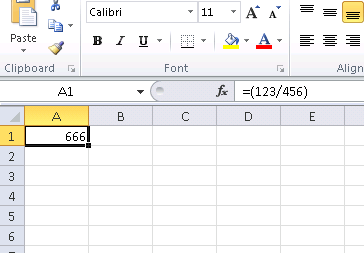
\includegraphics[width=0.6\textwidth]{digging_into_code/Excel_prank.png}
\caption{Der Scherz hat funktioniert}
\end{figure}

Wenn wir das gleiche mit der selben Excel Version versuchen, jedoch in 64-Bit Umgebungen.
Dann finden wir nur noch 12 \FDIV Instruktionen und die Instruktion nach der wir suchen ist
die dritte. 

\begin{lstlisting}
tracer.exe -l:excel.exe bpx=excel.exe!BASE+0x1B7FCC,set(st0,666)
\end{lstlisting}

\myindex{x86!\Instructions!DIVSD}

Es sieht danach aus als w\"aren viele der Division Operationen der \Tfloat und \Tdouble Typen, vom Compiler mit SSE Instruktionen ersetzt wurden.
Wie z.B \TT{DIVSD} (\TT{DIVSD} kommt insgesamt 268 mal vor).

\mysection{Verd\"achtige Code muster}

\subsection{XOR Instruktionen}
\myindex{x86!\Instructions!XOR}

Instruktionen wie \TT{XOR op, op} (zum Beispiel, \TT{XOR EAX, EAX})
werden normal daf\"ur benutzt Register Werte auf Null zu setzen, wenn jedoch
einer der Operanden sich unterscheidet wird die \q{exclusive or} Operation 
ausgef\"uhrt.

Diese Operation wird allgemeinen selten benutzt beim programmieren, aber ist
weit verbreitet in der Kryptografie, besonders bei Amateuren der Kryptografie.
Sowas ist besonders Verd\"achtig wenn der zweite Operand eine große Zahl ist.

Das k\"onnte ein Hinweis sein das etwas ver-/entschl\"usselt wird oder Checksumme berechnet werden, etc.

Eine Ausnahme dieser Beobachtung ist der \q{canary} (\myref{subsec:BO_protection}). 
Die Generierung und das pr\"ufen des \q{canary} werden oft mit Hilfe der \XOR Instruktion gemacht. 

\myindex{AWK}

Dieses AWK Skript kann benutzt werden um \IDA{} listing (.lst) Dateien zu parsen:

\lstinputlisting{digging_into_code/awk.sh}

Es sollte auch noch erw\"ahnt werden das diese Art von Skript in der Lage ist inkorrekt disassemblierten Code zu erkennen
(\myref{sec:incorrectly_disasmed_code}).

\subsection{Hand geschriebener Assembler code}

\myindex{Function prologue}
\myindex{Function epilogue}
\myindex{x86!\Instructions!LOOP}
\myindex{x86!\Instructions!RCL}

Moderne Compiler benutzen keine \TT{LOOP} und \TT{RCL} Instruktionen.
Auf der anderen Seite sind diese Instruktionen sehr beliebt bei Programmieren die Code direkt in Assembler schreiben.
Wenn man diese Instruktionen sieht, kann man mit hoher Sicherheit sagen das dieses Code Fragment h\"andisch geschrieben wurde.,
Diese Instruktionen sind in der Instruktionsliste im Anhang mit (M) markiert: \myref{sec:x86_instructions}.

\par Die Funktions Prolog und Epilog sind allgemein nicht vorhanden bei handgeschriebenen Assembler Code.

\par Tats\"achlich gibt es kein bestimmtes System um Argumente an Funktionen zu \"ubergeben wenn der Code handgeschrieben wurde. 

\par Beispiel aus dem Windows 2003 Kernel (ntoskrnl.exe file):

\lstinputlisting[style=customasmx86]{digging_into_code/ntoskrnl.lst}

Tats\"achlich, wenn wir in den \ac{WRK} v1.2 source code schauen, kann dieser Code einfach in der Datei
\emph{WRK-v1.2\textbackslash{}base\textbackslash{}ntos\textbackslash{}ke\textbackslash{}i386\textbackslash{}cpu.asm} gefunden werden.

% TBT
%\par 
%As of \INS{RCL}, I could find it in ntoskrnl.exe file from Windows 2003 x86 (MS Visual C compiler).
%It is occurred only once, in \TT{RtlExtendedLargeIntegerDivide()} function, and this might be inline assembler code case.

\mysection{Using magic numbers while tracing}

Oft ist unser Hauptziel zu verstehen wie ein Programm einen Wert behandelt der entweder \"uber eine Datei oder \"uber das Netzwerk erhalten wurde.
Das manuelle tracen eines Wertes ist meistens ein ziemlich arbeits-intensiver Task. Eine der einfachsten Techniken um Werte zu Tracen (auch wenn nicht 100\% verl\"asslich)
ist eigene \emph{magic number}'s zu benutzen. 

Das \"ahnelt ein wenig dem Vorgang beim R\"ontgen auf gewisser weise: ein radioaktives Kontrastmittel wird dem Patienten injeziert,
welches dann benutzt wird um die Gef\"asse des Patienten besser zu erkennen duch die R\"onthgenstahlung. Wie das blut bei 
gesunden Menschen in den Nieren gereinigt wird wenn das Kontrastmittel im Blut ist, man kann dann sehr einfach auf dem
Bild der Tomografie erkennen ob sich Nierensteine oder Tumore in den Nierenbefinden. 

Wir k\"onnen einfach eine 32-Bit Zahl nehmen z.B \TT{0xbadf00d}, oder ein Geburtsdatum wie \TT{0x11101979}
und diese 4-Byte Zahl wird an einem bestimmten Punkt in eine Datei geschrieben welche von dem Programm 
das wir untersuchen genutzt wird. 

\myindex{\GrepUsage}
\myindex{tracer}

Dann w\"ahrend das programm getraced wird mit \tracer im \emph{code coverage} modus, mit der Hilfe von \emph{grep}
oder durch einfaches durchsuchen der Textdatei (der trace Ergebnisse), k\"onnen wir ganz einfach sehen wo der 
Wert benutzt wurde und wie er benutzt wurde. 

Beispiel der \emph{grepable} \tracer Ergebnissen im \emph{cc} mode:

\begin{lstlisting}[style=customasmx86]
0x150bf66 (_kziaia+0x14), e=       1 [MOV EBX, [EBP+8]] [EBP+8]=0xf59c934 
0x150bf69 (_kziaia+0x17), e=       1 [MOV EDX, [69AEB08h]] [69AEB08h]=0 
0x150bf6f (_kziaia+0x1d), e=       1 [FS: MOV EAX, [2Ch]] 
0x150bf75 (_kziaia+0x23), e=       1 [MOV ECX, [EAX+EDX*4]] [EAX+EDX*4]=0xf1ac360 
0x150bf78 (_kziaia+0x26), e=       1 [MOV [EBP-4], ECX] ECX=0xf1ac360 
\end{lstlisting}
% TODO: good example!

Das gleiche verfahren kann man auch auf Netzwerkpakete anwenden.
F\"ur die \emph{magic number} ist es wichtig das diese einzigartig ist und nicht im Programm code vorkommt.

\newcommand{\DOSBOXURL}{\href{http://blog.yurichev.com/node/55}{blog.yurichev.com}}

\myindex{DosBox}
\myindex{MS-DOS}
Neben dem \tracer Befehl, gibt es noch den DosBox (MS-DOS emulator) im heavydebug Modus,
welcher in der Lage ist alle Informationen \"uber alle Register zust\"ande f\"ur jede ausgef\"uhrte Instruktion des Programmes in
eine einfache Textdatei\footnote{See also my blog post about this DosBox feature: \DOSBOXURL{}} zu schreiben, so kann
diese Technik f\"ur DOS Programme n\"utzlich sein. 


\mysection{Schleifen}

Wann immer ein Programm mit einer Datei oder einem Puffer bestimmter Größe
zu tun hat, muss dies eine Art von Verabeitungsschleife im code haben.

Dies ist ein reales Beispiel der \tracer-Tool-Ausgabe, bei dem der Code auf
irgendeine Weise codierte Datei von 258 Byte lud.
Das Tool lief mit der Absicht die Zahl der Anweisungen zukommen
(ein \ac{DBI}-Tool würde dies heutzutage sehr viel besser machen).
Ich fand sehr schnell ein Code-Stück, welches 259/258 mal ausgeführt wurde.

\lstinputlisting{digging_into_code/crypto_loop.txt}

Wie sich herausstellte war dies auch eine Decodier-Schleife.

\mysection{x86}

\subsection{Terminologie}

Geläufig für 16-Bit (8086/80286), 32-Bit (80386, etc.), 64-Bit.

\myindex{IEEE 754}
\myindex{MS-DOS}
\begin{description}
	\item[Byte] 8-Bit.
		Die DB Assembler-Direktive wird zum Definieren von Variablen und Arrays genutzt.
		Bytes werden in dem 8-Bit-Teil der folgenden Register übergeben:
		\TT{AL/BL/CL/DL/AH/BH/CH/DH/SIL/DIL/R*L}.
	\item[Wort] 16-Bit.
		DW Assembler-Direktive \dittoclosing.
		Bytes werden in dem 16-Bit-Teil der folgenden Register übergeben:
			\TT{AX/BX/CX/DX/SI/DI/R*W}.
	\item[Doppelwort] (\q{dword}) 32-Bit.
		DD Assembler-Direktive \dittoclosing.
		Doppelwörter werden in Registern (x86) oder dem 32-Bit-Teil der Register (x64) übergeben.
		In 16-Bit-Code werden Doppelwörter in 16-Bit-Registerpaaren übergeben.
	\item[zwei Doppelwörter] (\q{qword}) 64-Bit.
		DQ Assembler-Direktive \dittoclosing.
		In 32-Bit-Umgebungen werden diese in 32-Bit-Registerpaaren übergeben.
	\item[tbyte] (10 Byte) 80-Bit oder 10 Bytes (für IEEE 754 FPU Register).
	\item[paragraph] (16 Byte) --- Bezeichnung war in MS-DOS Umgebungen gebräuchlich.
\end{description}

\myindex{Windows!API}

Datentypen der selben Breite (BYTE, WORD, DWORD) entsprechen auch denen in der Windows \ac{API}.

% TODO German Translation (DSiekmeier)
%\input{appendix/x86/registers} % subsection
%\input{appendix/x86/instructions} % subsection
\subsection{npad}
\label{sec:npad}

\RU{Это макрос в ассемблере, для выравнивания некоторой метки по некоторой границе.}
\EN{It is an assembly language macro for aligning labels on a specific boundary.}
\DE{Dies ist ein Assembler-Makro um Labels an bestimmten Grenzen auszurichten.}
\FR{C'est une macro du langage d'assemblage pour aligner les labels sur une limite
spécifique.}

\RU{Это нужно для тех \emph{нагруженных} меток, куда чаще всего передается управление, например, 
начало тела цикла. 
Для того чтобы процессор мог эффективнее вытягивать данные или код из памяти, через шину с памятью, 
кэширование, итд.}
\EN{That's often needed for the busy labels to where the control flow is often passed, e.g., loop body starts.
So the CPU can load the data or code from the memory effectively, through the memory bus, cache lines, etc.}
\DE{Dies ist oft nützlich Labels, die oft Ziel einer Kotrollstruktur sind, wie Schleifenköpfe.
Somit kann die CPU Daten oder Code sehr effizient vom Speicher durch den Bus, den Cache, usw. laden.}
\FR{C'est souvent nécessaire pour des labels très utilisés, comme par exemple le
début d'un corps de boucle. Ainsi, le CPU peut charger les données ou le code depuis
la mémoire efficacement, à travers le bus mémoire, les caches, etc.}

\RU{Взято из}\EN{Taken from}\DE{Entnommen von}\FR{Pris de} \TT{listing.inc} (MSVC):

\myindex{x86!\Instructions!NOP}
\RU{Это, кстати, любопытный пример различных вариантов \NOP{}-ов. 
Все эти инструкции не дают никакого эффекта, но отличаются разной длиной.}
\EN{By the way, it is a curious example of the different \NOP variations.
All these instructions have no effects whatsoever, but have a different size.}
\DE{Dies ist übrigens ein Beispiel für die unterschiedlichen \NOP-Variationen.
Keine dieser Anweisungen hat eine Auswirkung, aber alle haben eine unterschiedliche Größe.}
\FR{À propos, c'est un exemple curieux des différentes variations de \NOP. Toutes
ces instructions n'ont pas d'effet, mais ont une taille différente.}

\RU{Цель в том, чтобы была только одна инструкция, а не набор NOP-ов, 
считается что так лучше для производительности CPU.}
\EN{Having a single idle instruction instead of couple of NOP-s,
is accepted to be better for CPU performance.}
\DE{Eine einzelne Idle-Anweisung anstatt mehrerer NOPs hat positive Auswirkungen
auf die CPU-Performance.}
\FR{Avoir une seule instruction sans effet au lieu de plusieurs est accepté comme
étant meilleur pour la performance du CPU.}

\begin{lstlisting}[style=customasmx86]
;; LISTING.INC
;;
;; This file contains assembler macros and is included by the files created
;; with the -FA compiler switch to be assembled by MASM (Microsoft Macro
;; Assembler).
;;
;; Copyright (c) 1993-2003, Microsoft Corporation. All rights reserved.

;; non destructive nops
npad macro size
if size eq 1
  nop
else
 if size eq 2
   mov edi, edi
 else
  if size eq 3
    ; lea ecx, [ecx+00]
    DB 8DH, 49H, 00H
  else
   if size eq 4
     ; lea esp, [esp+00]
     DB 8DH, 64H, 24H, 00H
   else
    if size eq 5
      add eax, DWORD PTR 0
    else
     if size eq 6
       ; lea ebx, [ebx+00000000]
       DB 8DH, 9BH, 00H, 00H, 00H, 00H
     else
      if size eq 7
	; lea esp, [esp+00000000]
	DB 8DH, 0A4H, 24H, 00H, 00H, 00H, 00H 
      else
       if size eq 8
        ; jmp .+8; .npad 6
	DB 0EBH, 06H, 8DH, 9BH, 00H, 00H, 00H, 00H
       else
        if size eq 9
         ; jmp .+9; .npad 7
         DB 0EBH, 07H, 8DH, 0A4H, 24H, 00H, 00H, 00H, 00H
        else
         if size eq 10
          ; jmp .+A; .npad 7; .npad 1
          DB 0EBH, 08H, 8DH, 0A4H, 24H, 00H, 00H, 00H, 00H, 90H
         else
          if size eq 11
           ; jmp .+B; .npad 7; .npad 2
           DB 0EBH, 09H, 8DH, 0A4H, 24H, 00H, 00H, 00H, 00H, 8BH, 0FFH
          else
           if size eq 12
            ; jmp .+C; .npad 7; .npad 3
            DB 0EBH, 0AH, 8DH, 0A4H, 24H, 00H, 00H, 00H, 00H, 8DH, 49H, 00H
           else
            if size eq 13
             ; jmp .+D; .npad 7; .npad 4
             DB 0EBH, 0BH, 8DH, 0A4H, 24H, 00H, 00H, 00H, 00H, 8DH, 64H, 24H, 00H
            else
             if size eq 14
              ; jmp .+E; .npad 7; .npad 5
              DB 0EBH, 0CH, 8DH, 0A4H, 24H, 00H, 00H, 00H, 00H, 05H, 00H, 00H, 00H, 00H
             else
              if size eq 15
               ; jmp .+F; .npad 7; .npad 6
               DB 0EBH, 0DH, 8DH, 0A4H, 24H, 00H, 00H, 00H, 00H, 8DH, 9BH, 00H, 00H, 00H, 00H
              else
	       %out error: unsupported npad size
               .err
              endif
             endif
            endif
           endif
          endif
         endif
        endif
       endif
      endif
     endif
    endif
   endif
  endif
 endif
endif
endm
\end{lstlisting}
 % subsection

% FIXME comparison!
\subsection{Memory \q{snapshots} comparing}
\label{snapshots_comparing}

Die Technik zwei Memory Snapshots zu vergleichen ist recht einfach, das hat man auch oft benutzt um 8-Bit Computerspiele und
\q{high score}'s  zu hacken.

Zum Beispiel, wenn man ein geladenes Spiel auf einem 8-Bit Computer hat ( auf den Maschinen ist nicht viel Speicher 
vorhanden, jedoch braucht das Spiel noch weniger Speicher) und du weißt was du im Spiel hast, sagen wir 100 Patronen, 
nun kann man einen \q{snapshot} vom gesamten Speicher machen und diesen Irgendwohin speichern. Dann verschiesst man 
eine Patrone, dann geht der Patronen Z\"ahler auf 99, nun erstellt man den zweiten Snapshot und Vergleich die beiden: 
Nun muss es irgendwo ein Byte geben das vorher 100 war und jetzt 99 ist. 

Betrachtet man den Fakt das diese 8-Bit Spiele oftmals in Assembler geschrieben wurden und diese Variablen meist global 
waren, konnte man ziemlich einfach bestimmen welche Adressen im Speicher den Kugelz\"ahler beinhalten. Wenn man nach allen 
Referenzen der Adresse im dissassembelten Spiel code sucht, ist es nicht schwer den Code \glslink{decrement}{decrementing} 
zu finden und dann eine \gls{NOP} Instruktion an diese Stelle zu schreiben, oder gar mehrere \gls{NOP}-s, und dann hat man 
ein Spiel bei dem man f\"ur immer 100 Kugeln hat. %<-- das kacke der ganze block
\myindex{BASIC!POKE}
Spiele auf 8-Bit Computern wurden allgemein an konstanten Adressen geladen, zus\"atzlich gab es nicht viele unterschiedliche
Versionen des Spiels (  Es war meist eine Version f\"ur lange Zeit popul\"ar ), dadurch wussten enthusiastische Gamer welche
Bytes (durch das benutzen von Basic Instruktionen wie \gls{POKE}) \"uberschrieben werden mussten um das Spiel zu hacken. 
Das hat wiederum zu \q{cheat} listen gef\"uhrt die in Magazinen f\"ur 8-Bit Games erschienen, die dann \gls{POKE} Instruktionen enthielten.

% Considering the fact that these 8-bit games were often written in assembly language and such variables were global,
% it can be said for sure which address in memory has holding the bullet count. If you searched for all references to the
% address in the disassembled game code, it was not very hard to find a piece of code \glslink{decrement}{decrementing} the bullet count,
% then to write a \gls{NOP} instruction there, or a couple of \gls{NOP}-s, 
% and then have a game with 100 bullets forever.
% \myindex{BASIC!POKE}
% Games on these 8-bit computers were commonly loaded at the constant
% address, also, there were not much different versions of each game (commonly just one version was popular for a long span of time),
% so enthusiastic gamers knew which bytes must be overwritten (using the BASIC's instruction \gls{POKE}) at which address in
% order to hack it. This led to \q{cheat} lists that contained \gls{POKE} instructions, published in magazines related to
% 8-bit games.

\myindex{MS-DOS}

Es ist auch einfach \q{high score} Dateien zu modifizieren, das funktioniert nicht nur bei 8-Bit Spielen. Man achte 
auf seinen Highscore Z\"ahler, dann macht man ein Backup der Datei. Wenn sich der \q{high score} Z\"ahler \"andert, vergleicht man die 
zwei Dateien miteinander, das kann man sogar mit dem DOS Tool FC\footnote{MS-DOS Utility zum vergleichen von  Dateien} (\q{high score} Dateien,
sind oft in Bin\"arer Form). 

Es wird beim Vergleichen der Dateien einen Punkt geben wo einige Bytes sich unterscheiden und 
es wird leicht sein, die Punkte zu sehen die die Bytes des Punktez\"ahler beinhalten. 
Jedoch sind sich die Spiele Entwickler solcher Tricks bewusst und bauen Wege ein um das Programm
vor solchen Manipulationen zu sch\"utzen. 

Ein \"ahnliches Beispiel findet man auch in dem Buch \myref{Millenium_DOS_game}.

% TODO: пример с какой-то простой игрушкой?

% TBT 

\subsubsection{Windows registry}

Es ist auch m\"oglich die Windows Regestry zu vergleichen vor und nach der Programm Installation.

Es ist eine sehr popul\"are Methode Regestry Elemente zu finden die vom Programm benutzt werden.
Vielleicht ist das auch der Grund warum die \q{windows regestry cleaner} Shareware so popul\"ar ist.

% TBT

\subsubsection{Blink-comparator}

Der Vergleich von Datei- oder Speichersnapshots erinnert ein wenig an einen Blinkkomparator
\footnote{\url{https://en.wikipedia.org/wiki/Blink_comparator}}
ein Ger\"at das in der Vergangenheit von Astronomen benutzt wurde, um sich bewegende Astronomische
Objekte zu finden.

Ein Blinkkomperator erlaubt es schnell zwischen Photographie zu wechseln die zu unterschiedlicher
Zeit aufgenommen wurden, so kann ein Astronom Unterschiede zwischen Fotografien visuell erkennen.

Ach \"ubrigens, Pluto wurde durch einen solchen Blink-Komparator 1930 entdeckt.

% TBT \input{digging_into_code/ISA_detect_DE}

\mysection{Andere Dinge}

\subsection{Die Idee}  

Ein Reverse Engineer sollte versuchen so oft wie m\"oglich in den Schuhen des
Programmierers zu laufen. Um ihren/seinen Standpunkt zu betrachten uns sich
selbst zu Fragen wie man einen Task in spezifischen F\"allen l\"osen w\"urde.

\subsection{Anordnung von Funktionen in Bin\"ar Code}  

S\"amtliche Funktionen die in einer einzelnen .c oder .cpp-Datei gefunden werden,
werden zu den entsprechenden Objekt Dateien (.o) kompiliert. Sp\"ater, f\"ugt
der Linker alle Objektdatein die er braucht zusammen, ohne die Reihenfolge oder
die Funktionen in Ihnen zu ver\"andern. Als eine Konsequenz, ergibt sich daraus
wenn man zwei oder mehr aufeinander folgende Funktionen sieht, bedeutet dass das
sie in der gleichen Source Code Datei platziert waren (Außer nat\"urlich man bewegt
sich an der Grenze zwischen zwei Dateien.). Das bedeutet das diese Funktionen etwas
gemeinsam haben, das sie aus dem gleichen \ac{API}-Level stammen oder aus der
gleichen Library, etc.

% TBT
%\myindex{CryptoPP}
%This is a real story from practice: once upon a time, the author searched for Twofish-related functions in
%a program with CryptoPP library linked, especially encryption/decryption functions.\\
%I found the \verb|Twofish::Base::UncheckedSetKey()| function, but not others.
%After peeking into the \verb|twofish.cpp| source code
%\footnote{\url{https://github.com/weidai11/cryptopp/blob/b613522794a7633aa2bd81932a98a0b0a51bc04f/twofish.cpp}}, it became clear that all functions are located in one module (\verb|twofish.cpp|).\\
%So I tried all function that followed \verb|Twofish::Base::UncheckedSetKey()|---as it happened,\\
%one was \verb|Twofish::Enc::ProcessAndXorBlock()|, another---\verb|Twofish::Dec::ProcessAndXorBlock()|.

\subsection{kleine Funktionen} 

Sehr kleine oder leere Funktionen  (\myref{empty_func})
oder Funktionen die nur ``true'' (1) oder ``false'' (0) (\myref{ret_val_func}) sind weit verbreitet,
und fast jeder ordentlicher Compiler tendiert dazu nur solche Funktionen in den resultierenden ausf\"uhrbaren Code zu stecken,
sogar wenn es mehrere gleiche Funktionen im Source Code bereits gibt. 
Also, wann immer man solche kleinen Funktionen sieht die z.B nur aus \TT{mov eax, 1 / ret} bestehen und von mehreren 
Orten aus referenziert werden (und aufgerufen werden k\"onnen), und scheinbar keine Verbindung zu einander haben, dann 
ist das wahrscheinlich das Ergebnis einer Optimierung. 

\subsection{\Cpp}

\ac{RTTI}~(\myref{RTTI})-data ist vielleicht auch n\"utzlich f\"ur die \Cpp Klassen Identifikation.
